\section{Algorithm for checking language emptiness}

\begin{example}
  \( \forall x.\ \forall y.\ -2 x + 3y = 1 \Rightarrow (\exists z.\ x -3z = 1) \wedge (\exists z.\ y -2z = 1) \)
  \begin{figure}
    \caption{Equation \( -2 x + 3y = 1 \)}
    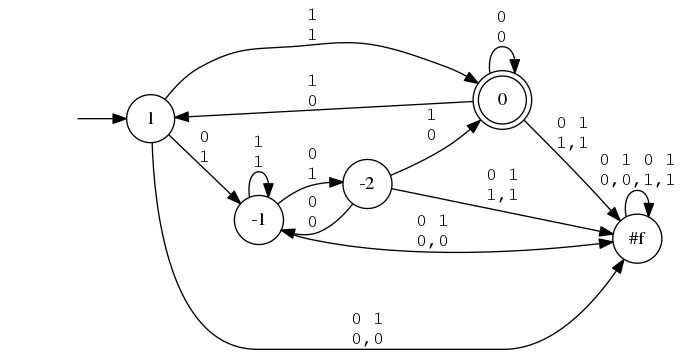
\includegraphics[width=10cm]{images/eq5.png}
  \end{figure}
  \begin{figure}
    \caption{Equation \( x -3z = 1 \) and \( \exists z.\ x -3z = 1 \)}
    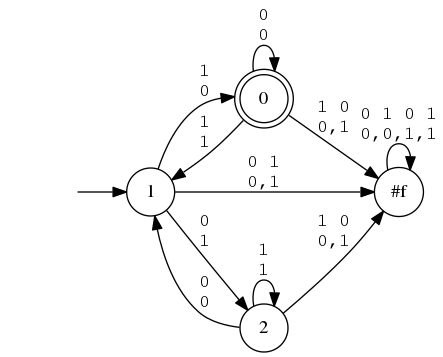
\includegraphics[width=8cm]{images/mod3is1_x.png}
    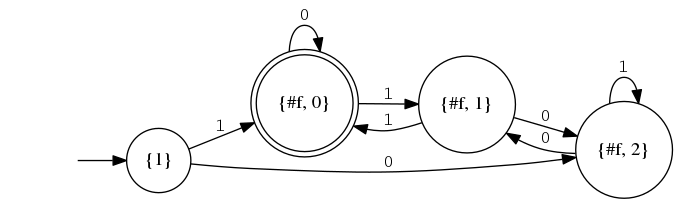
\includegraphics[width=10cm]{images/proj_mod3is1_x.png}
  \end{figure}
  \begin{figure}
    \caption{Equation \( y -2z = 1 \) and \( \exists z.\ y -2z = 1 \)}
    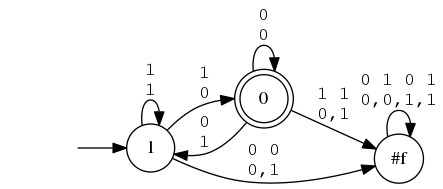
\includegraphics[width=8cm]{images/odd_x.png}
    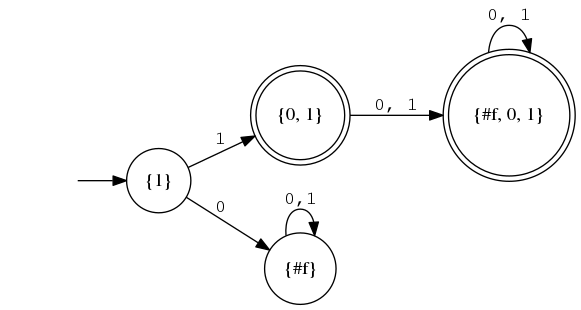
\includegraphics[width=10cm]{images/proj_odd_x.png}
  \end{figure}
  \begin{figure}
    \caption{AFA for \( -2 x + 3y = 1 \)}
    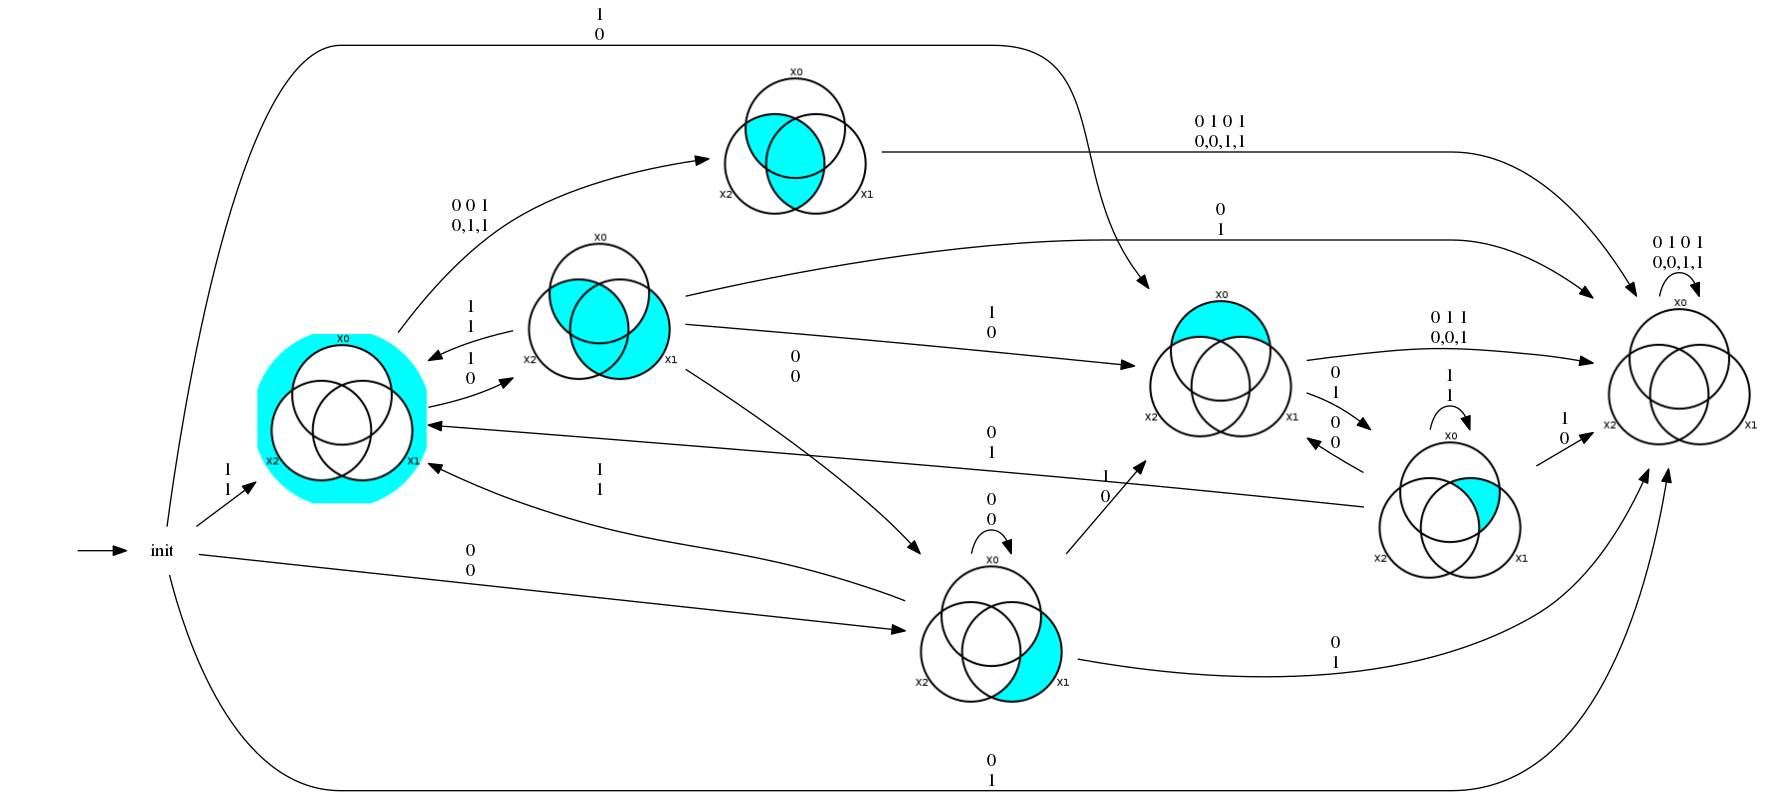
\includegraphics[width=10cm]{images/afa_eq5.png}
  \end{figure}
  \begin{figure}
    \caption{AFA for \( x -3z = 1 \)}
    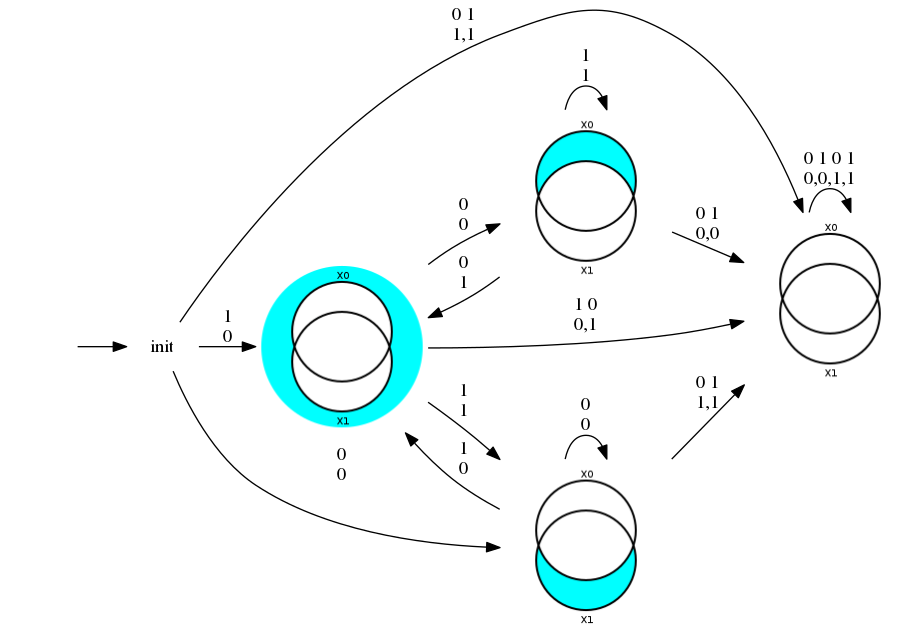
\includegraphics[width=10cm]{images/afa_mod3is1_x.png}
  \end{figure}
  \begin{figure}
    \caption{AFA for \( y -2z = 1 \)}
    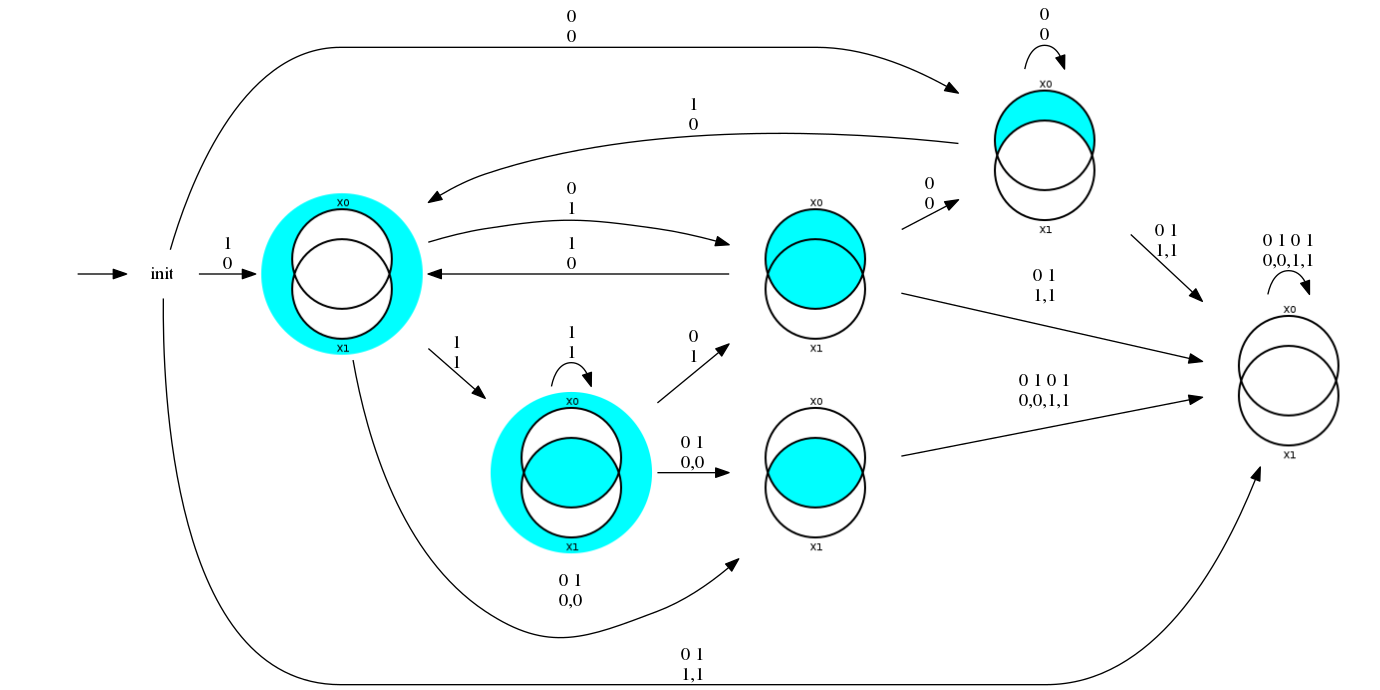
\includegraphics[width=10cm]{images/afa_odd_x.png}
  \end{figure}
\end{example}
\iffalse
Given an \( \mathit{AFA}\) \( \mathcal{A} \), the \textit{emptiness} problem is
to determine \( \mathcal{L}(\mathcal{A}) = \varnothing \).

\begin{definition}
  \begin{align*}
    \mathit{EC}(\Gamma) :=
    \begin{dcases}
    \Gamma \cup \Gamma'              &\text{if } f \models \Gamma \cup \Gamma'
    \\
    \Gamma                           &\text{if } \Gamma \supseteq \Gamma'
    \\
    \mathit{EC}(\Gamma \cup \Gamma') &\text{otherwise } 
    \end{dcases}
    \\
    \text{ where, } \Gamma' :=
    \bigcup\limits_{\alpha \in \Gamma}
    \bigcup\limits_{c \in \Sigma}
    \{ \beta \mid \alpha \xrightarrow[]c \beta \}
    \tag{EC}
  \end{align*}
\end{definition}

\begin{example}
\( \mathit{EC}(\{ q_0 \}) = \{ q_0, 0, q_1 \wedge q_2, \neg q_1 \wedge q_2 \} \).
\end{example}

\begin{definition}
Replace (EC) with (AC) and we have the \( \mathit{antichain} \) algorithm. 
    \begin{align*} \cdots & \text{ where, } \Gamma' :=
    \bigcup\limits_{\alpha \in \Gamma}
    \bigcup\limits_{c \in \Sigma}
    \{
    \beta \mid \alpha \xrightarrow[]c \beta
    \wedge
    \forall \gamma \in \Gamma .\ \beta \not \Rightarrow \gamma
    \}
    \tag{AC}
    \end{align*}
\end{definition}

We say \( \alpha \) and \( \beta \) are congruent if the language beginning from
\( \alpha \) and from \( \beta \) are the same and denote \( \alpha \cong
\beta\).

\begin{definition}
  \begin{align*} \cdots & \text{ where, } \Gamma' :=
    \bigcup\limits_{\alpha \in \Gamma}
    \bigcup\limits_{c \in \Sigma}
    \{
    \beta \mid \alpha \xrightarrow[]c \beta
    \wedge
    \forall \gamma \in \Gamma .\ \beta \not \cong \gamma
    \}
    \tag{CC}
  \end{align*}
\end{definition}

\begin{theorem}
  \begin{itemize}
  \item \(EC(\{s\}) \models \text{ iff }
    \mathcal{L}(\mathcal{A}) \neq \varnothing. \)
  \item \(AC(\{s\}) \models \lceil \text{ iff }
    \mathcal{L}(\mathcal{A}) \neq \varnothing. \)
  \item \(CC(\{s\}) \models \lceil \text{ iff }
    \mathcal{L}(\mathcal{A}) \neq \varnothing. \)
\end{itemize}
\end{theorem}
\fi
